%        File: learnability.tex
%     Created: Mon Feb 06 11:00 AM 2017 E
% Last Change: Mon Feb 06 11:00 AM 2017 E
%
% arara: pdflatex: {options: "-draftmode"}
% arara: biber
% arara: pdflatex: {options: "-draftmode"}
% arara: pdflatex: {options: "-file-line-error-style"}
\documentclass[MilwayThesis]{subfiles}

\begin{document}
In this section, I will evaluate some previous analyses of resultatives, based on their learnability, largely setting aside questions of over-/under-generation.
This choice of evaluation metric is motivated by the overall goals of this thesis and by the fact that questions of generative capacity are well-addressed by the analyses that I will evaluate.

The resultative parameter presents an acquisition problem for two broad reasons.
The first problem is that, on the surface, resultatives, which are parameterized, are indistinguishable from depictives, which appear to be universal.
The two construction types are indistinguishable in the sense that both correspond to the string template in \Next (modulo independent word order variation).
\ex. \textsc{Subj} V \textsc{Obj} Adj.

This indistinguishability is evident in the fact that one can construct examples which are truly ambiguous between resultative and depictive readings, as in \Next.
\ex. 
\a. He fried the fish dry.
\a. $\approx$ He fried the fish once it was dry. (\textbf{Depictive})
\b. $\approx$ He fried the fish until it was dry. (\textbf{Resultative})
\z.
\b. She painted the barn red.
\a. $\approx$ The barn is red in her painting. (\textbf{Depictive})
\b. $\approx$ She applied a coat of red paint to the door. (\textbf{Resultative})
\z.

Assuming a child acquiring either French or English encounters sentences with the form of \LLast in their PLD, there is no obvious way for the child to determine whether a given secondary predicate is to be interpreted depictively or resultatively.

An empiricist might object, arguing that the ambiguous examples above are highly constructed, and would easily by disambiguated in context.
They would insist that the learner would infer a positive setting of the resultative parameter from the use of a secondary predication construction in the presence of a resultative event.
So, an English learner, but not a French learner, might be exposed to the context-sentence pairing in \Next.
\ex. 
\a.[\textbf{Context:} ] A woman is methodically hammering a lump of metal.
A parent draws their child's attention to the hammering event and utters:
\b.[\textbf{A:}] She's hammering the metal flat.

Even this, however, is not fully unambiguous.
While it certainly couldn't be interpreted as a depictive, \textit{flat} could be interpreted as a manner adverb, modifying \textit{hammering}.
Such unavoidable ambiguity would make it difficult to employ any sort of semantic bootstrapping in the acquisition of the resultative parameter.

The second problem comes from the fact that both English-type and French-type languages can express resultative semantics periphrastically as in \Next.
\ex. (periphrasis)

The resultative parameter, then, is a one-or-both parameter, unlike other parameters which are either/or choices.
The verb raising parameter, for instance, is an either/or choice which can be made on the basis of the PLD:
If a learner encounters subject-verb inversion, they can infer that \textit{do}-support is impossible (at least for a given verb or verb class). 
If, however, a learner encounters \textit{do}-support, they can infer that subject-verb inversion is impossible. 
Turning to the resultative parameter, no such inference available to the learner:
The presence of a periphrastic resultatives in no way implies the impossiblity of adjectival resultatives, and vice versa.

One approach to the resultative parameter is what I will call the lexicalization account.
Under this account, event descriptions are decomposable into several universal features (\textit{e.g.}, \textsc{Result}, \textsc{Manner}, \textsc{Process}), and language variation results from languages lexicalizing these features differently.
One such an account by \textcite{son2008microparameters} proposes that English and German lexicalize \textsc{Result} in null heads, while Romance languages only lexicalize \textsc{Result} in verbs.
\ex.
\raisebox{-.9\height}{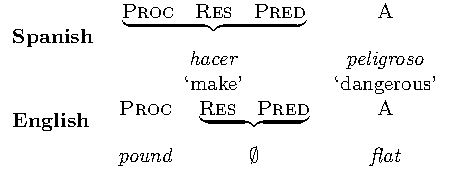
\includegraphics{lexicalization_table}}

Since the null LI is restricted to resultatives, the task of acquiring it depends on the learner distinguishing resultatives from depictives, and, as discussed above, such a task is far from trivial.

Indirect acquisition accounts of the resultative parameter, on the other hand, do not (necessarily) suffer from the drawbacks of direct acquisition.
The two that I will discuss -- \textcite{beck2001complex} and \textcite{kratzer_building_2004} -- both take Snyder's (\citeyear{snyder1995language}) compounding parameter as a starting point, but propose different sources of parameterization.



\end{document}
